%-------------------------------------------------------------------------------
\section{Introduction}
%-------------------------------------------------------------------------------

Web application companies face increasing legal requirements to protect users’ data. These
requirements pressure companies to properly delete and anonymize users' data when a user requests to
\emph{unsubscribe} from the service (i.e.,\ revoke access to their personal data). For example, the
GDPR requires that any data remaining after a user unsubscribes cannot be (directly or
indirectly) used to identify the user~\cite{gdpr}.  

In this paper, we propose \sys{}, which enables application developers to specify fine-grained
privacy policies to meet de-identification requirements, and goes beyond: with \sys{}, it is
possible for users to switch between a privacy-preserving unsubscribed mode and an
identity-revealing subscribed mode at any time without permanently losing their data. This
facilitates important new web service paradigms, such as users granting a time-limited ``lease'' of
data to a service instead of having a permanent service account.

Developers using \sys{} specify privacy-sensitive data and the state of such data after the user
leaves. \sys{} \emph{decorrelates} a user's data according to this specification when a user unsubscribes;
post-decorrelation application state is guaranteed to match the specification.  When a user wishes
to resubscribe, \sys{} \emph{recorrelates} the user's data with the user, restoring the user to her
original subscribed state as much as possible. 

\sys{} makes the key observation that a user's data entities (e.g.,\ posts and upvotes) can leak identifying
information in two ways: (1) directly via its content, and (2) indirectly via the correlations it has to
other data entities in the system.  
Correlations can range from obviously identifying (e.g.,\ posts correlated
with a user clearly belong to that user), to subtly perilous: posts correlated with a
particular user-generated tag most likely belong to the tag's author, and posts liked by the  
same group of users likely belong to a friend of the group. 

Many web applications (e.g.,\ Lobst.rs and Reddit) have come up with solutions to de-identify direct
content by anonymizing unique identifiers, leaving arbitrary user-generated content out of scope.
Other applications (e.g.,\ Facebook and Twitter) delete (most of the) user's data. The former
optimizes the amount of data the application keeps, but also retains all correlations between data
entities; the latter can lead to confusing semantics for the application (e.g.,\ nonsensical comment
threads) and the loss of useful application data. In both cases, accounts cannot be restored after
deletion.
\lyt{Applications such as Facebook or Twitter do support user account deactivation by hiding (most) of the
user's data, but retain all user data with their identifiers in their databases.}

Developers using \sys{} can specify policies that both anonymize unique identifiers, and remove
identifying information stemming from correlations between data entities. \sys{}'s support for
fine-grained decorrelation policies gives developers options beyond either completely retaining
these links or deleting of all of the user's data and their dependees (while still supporting
these options). The complexity of implementating such policies is hidden from the developer:
\sys{} automatically performs decorrelation in a way that allows for recorrelation upon
resubscription, while still achieving performance comparable to today’s widely-used databases and
requiring no modification of application schemas. 

\subsection{The goal of decorrelation}
Decorrelation ideally breaks connections between data entities that would otherwise allow
an adversary to determine that two entities belong to the same (unsubscribed) user:
post-decorrelation, an adversary should not be able to distinguish between a scenario in which two data entities
have been generated by two distinct users, and one in which they were both generated by the same
(unsubscribed) user.  If two of a user's entities cannot be correlated back to the user, then at
most one of these entities may leak identifying information about the user.\footnote{Assume for a
contradition that both entities leak identifying information: then both entities are more likely to
have been generated by a particular identity than any other, contradicting our assumption.}  Thus,
if the content of individual data entities is appropriately anonymized, then perfect decorrelation prevents
identifying information from being leaked via correlations.

\subsubsection{Threat Model} 
An adversary aims to relink decorrelated entities to unsubscribed users after \sys{}
performs decorrelation. We make the following assumptions about such an adversary: 
\begin{itemize}
    \item An adversary can perform only those queries allowed by the application API, 
i.e.,\ can access the application only via its public interface. 
%\lyt{Alternatively, an adversary could perform arbitrary queries on some public subset of the
%application schema (e.g., all tables other than the mapping table, or all tables marked with some
%compliance policy); arbitrary queries over the
%entirety of the table are out of scope, unless ``private'' tables are removed and stored by
%unsubscribing users.}

    \item An adversary cannot perform application queries to the past or search web archives:
    information from prior application snapshots may reveal 
    exactly how data records were decorrelated from unsubscribed users. 

    \item An adversary cannot gain identifying information from arbitrary user-generated content (for
        example, a reposted screenshot, or text in user stories or comments). Decorrelation seeks to
        remove identifying information from user-generated data that can be enumerated or follows a
        specific pattern (e.g., a birthday or email address), and application metadata (e.g., date
        of postings, database ID columns).
\end{itemize}

\subsubsection{Problems with decorrelation taken too far.}
Decorrelation taken to the extreme breaks all correlations between entities recursively related to
the user being anonymized, replacing these correlations with ghost correlations.  This removes as
much correlation-based identifying information as possible while keeping data entities present, but
in practice, completely decorrelated data entities may be useless to the application.  Applications
may lack a meaningful way to generate ghost entities: what does it mean for a story to become many
ghost stories?  And even if ghosts can be generated, the noise and data pollution from ghost
entities may instead affect the accuracy and semantics of the application: users may see meaningless
content, comment threads may be disjoint and scattered, and highly-ranked content may suddenly lose
votes. 
%On the other extreme, however, performing no decorrelation at all fails to adequately de-identify

\sys{} offers developers a way to decorrelate as much as possible \emph{while still retaining
application semantics}. As the next section describes, \sys{} provides decorrelation specification
primitives with which developers can specify which (and how) entities can be decorrelated from other
entities, and which correlations must be kept for application correctness.

\subsection{Specifying Decorrelation Policies}
\lyt{FIGURE HERE} 

\begin{figure}
\begin{lstlisting}[language=Rust]
 pub enum GeneratePolicy {
     Random,
     Default,
     Custom(FnMut(ColumnValue) -> ColumnValue),
     ForeignKey, 
 }
 pub enum GhostColumnPolicy {
     CloneAll,
     CloneOne(gp: GeneratePolicy),
     Generate(gp: GeneratePolicy),
 }
 pub type GhostPolicy = 
    HashMap<Column, GhostColumnPolicy>;
 pub type EntityGhostPolicies = 
    HashMap<EntityName, GhostPolicy>;

pub enum DecorrelationPolicy {
     NoDecorRemove,
     NoDecorRetain,
     NoDecorSensitivity(f64),
     Decor,
 }
 pub struct KeyRelationship {
     child: EntityName,
     parent: EntityName,
     column_name: String,
     decorrelation_policy: DecorrelationPolicy,
 }
 pub type ApplicationPolicy = 
    (EntityGhostPolicies, Vec<KeyRelationship>);
\end{lstlisting}
    \caption{\sys{}-provided types to specify key relationships and ghost generation policies.
    \lyt{An actual instance of this policy is here: \url{https://github.com/tslilyai/gdpr/blob/master/decor/applications/lobsters/microbenchmarks/policy.rs}}}
\end{figure}

Application data is structured as tables, each representing a different \emph{table entity} type,
e.g.,\ stories, users, or votes. Table columns act as foreign keys to other table entities, or as
abstract keys that refer to abstract non-table entities (e.g.,\ a \texttt{thread\_id} comments column). 
Key relationships represent correlations between entity types.

\sys{} represents instances of key-based relationships between entities as the edges of a graph,
where the nodes are the entity instances: child entities are connected to parents via an instance of
a foreign or abstract key relationship. In the following, an \emph{edge} refers to an instance of a
foreign or abstract key relationship.

The developer provides a two-part specification to \sys{}: 
\begin{enumerate}
    \item Ghost entity generation policies on entity types, and
    \item Decorrelation policies for foreign/abstract key relationships specifying if and how
        instances of these edge types should be decorrelated.
\end{enumerate}

\noindent The following describes the options for the different parts of the developer-provided
specification in more detail.

\subsubsection{Ghost Entity Generation}
Developers can choose between the following ghost generation policies, which apply at 
per-column granularity.
\begin{itemize}
    \item \textbf{Cloned:} All ghosts have the same value as the original entity for this column.
        Recorrelation returns an entity with the original value.

    \item \textbf{Generated:} All ghosts have a generated value for this column. Generated values are
chosen to be random, a default value, or generated from the original value via a function provided by the developer.
        If the developer provides a reversible function (e.g.,\ has encrypted the original value
        with a user-specific key), then the original value is restored upon
        recorrelation; otherwise, recorrelation returns a generated value in place of the original.

        If the column represents a foreign key into another table, then either the referenced table must 
        have a ghost generation policy, or the foreign key is set to an existing entity or placeholder ghost (e.g.,
        the foreign key is set to point to ``deleted story''). It is up to the developer to ensure
        referential integrity in the latter case.

\item \textbf{Single Clone, Generated Remainder:} One ghost has the same value as the original
        entity; all other ghosts have generated values. Recorrelation returns an entity with the original value.
\end{itemize}


\subsubsection{Decorrelation Policies}

\paragraph{Policy 1: Decorrelate.}
Application developers specify that the relationship may be decorrelated.
\sys{} generates a ghost parent entity for the child entity according to the parent entity's ghost
generation policy, replacing the child's key with the new ghost parent key.

Resubscription (and recorrelation) removes any created ghost entities and restores the relationship
back to the original parent key instance.

%\lyt{There could also be an option to "decorrelate the minimum amount possible to reach a
%certain sensitivity threshold"; not sure if it's useful since the edges can already be
%decorrelated.}
%
\paragraph{Policy 2: Do not decorrelate.}
Application developers specify that this foreign or abstract key relationship cannot be decorrelated.
Developers select from the following subpolicy options: 
\begin{itemize}
    \item \textbf{Delete}: The child entity and its dependencies are deleted. This option should be
        selected if this type of key relationship cannot be decorrelated while retaining application
        semantics, but keeping the relationship would reveal too much identifying information.
        Upon recorrelation, however, these entities cannot be restored.

    \item \textbf{Retain}: Nothing is done on either side of the
        relationship. This option should only be selected if the developer knows that the
        relationship cannot leak identifying information.

    \item \textbf{Achieve sensitivity threshold $0 \le \sigma \le 1$}:
        A sensitivity threshold for an foreign/abstract key relationships specifies the maximum
        proportion of edge instances of a relationship type that may connect to \emph{sensitive}
        entities (i.e.,\ entities transitively correlated to the initial entity being decorrelated). 

        At a high level, the sensitivity threshold for a particular edge type estimates how much identifying
        information may leak from edge instances of that type.  For any given edge type, developers can
        determine an appropriate sensitivity threshold by approximating how much identifying information
        may be leaked if edges of this type with the same parent key \emph{all} correlate (even indirectly)
        back to the entity being decorrelated. In other words, what happens if all children of edges of this
        type (with the same parent) are sensitive?

        For example, consider the foreign key relationship from stories to tags. If all
        the stories tagged with the same parent tag in the entity graph were written by some
        (unsubscribed) user, would the story-tag correlation be problematic? The answer may be yes: 
        perhaps tags are customizable by the user, and any story with that tag will clearly
        belong to the unsubscribed user. In other cases, the answer may be no: even though the tag is only
        correlated with sensitive stories, the tag indicates nothing about who may have authored the stories.

        For many cases, the answer may lie somewhere in the middle: it is problematic if \emph{all} of
        children of edge of this type are sensitive, but perhaps it is acceptable if only a fraction of
        children of this edge type are sensitive. The maximum value for this fraction is the sensitivity threshold.
        For example, a reasonable sensitivity threshold might be $\sigma = 0.1$ for stories-tag key relationships:
        less than 10\% of all stories with a specific tag key should have been correlated (even
        indirectly) with an (unsubscribed) user. 

        \sys{} either generates ghost children entities with this edge type until the
        sensitivity threshold is met (if a ghost generation policy is specified for the child type); upon
        resubscription, \sys{} removes any generated ghost entities and edges.
        Note that if the generated ghosts are easily distinguished from actual entities, there is
        little privacy benefit from generating ghost entities to meet the threshold.

        If the children entity type has no associated ghost generation policy, \sys{} removes
        sensitive children and their dependencies until the threshold is met.  Upon recorrelation,
        however, these entities cannot be restored.

        If $\sigma = 0$, then this corresponds to removing all edges of this type
        with sensitive children (equivalent to a Delete policy); if $\sigma = 1$, \sys{} does
        nothing (equivalent to a Retain policy).
    \end{itemize}

\subsubsection{\sys{}'s Execution Algorithm}
Given this specification and an entity to be decorrelated as input, \sys{} acts as follows:
\begin{enumerate}
    \item \textbf{Parent-Child Traversal:} \sys{} traverses the entity graph starting from the input entity,
        going down parent to child edges (and halting if it detects a cycle).  As it traverses,
        \sys{} collects the edges it has traversed. 
    
    \item \textbf{Parent-Child Decorrelation:} Post-traversal, \sys{} acts on each edge instance
        according to the specified decorrelation relationship policy for that edge's type: if no
        policy is specified, \sys{} does nothing. If edges can be decorrelated, \sys{} generates
        ghost parent entities and new edges between child and ghost parent entities using the
        appropriate ghost entity generation policy. If edges cannot be decorrelated and should be
        retained or deleted, \sys{} does nothing or removes the child and edge respectively. 
    
        If there is a sensitivity threshold for the edge's type, \sys{} ensures the
        sensitivity of the edge is below $t$'s threshold, providing the edge type and the edge's
        parent key to the procedure described in Section~\ref{sensitivity_algo}. 

    \item \textbf{Child-Parent Decorrelation:} Next, \sys{} takes the children of all traversed edge
        instances, and considers the set of edges from these children to other parents
        \emph{not} traversed by \sys{} during the decorrelation phase. (In other words, these
        children entities have multiple key relationships to several parent entities, one of
        which is connected via a chain of parent-child edges to the input entity).

        Intuitively, children of edges traversed by \sys{} share a connection with the initial
        entity being decorrelated. Edges \emph{from} these children to other parent entities may
        thus leak sensitive identifying information. 

        \sys{} acts on these edges according to the specified decorrelation relationship policy for
        each edge's type. If these edges can be decorrelated, \sys{} generates ghost parent entities
        for each sensitive child.  If these edges cannot be decorrelated and should be retained or
        deleted, \sys{} does nothing or removes the child and edge respectively. 
        
        \lyt{Note: edge policies should take account the \emph{direction} of the edge
        (whether we're considering sensitive child->parent, or sensitive parent->child). We need
        this to allow policies that decorrelate a message from one unsubscribing user while still retaining the correlation
        to another subscribed user.}

        Otherwise, if there is a sensitivity threshold for the edge type, then \sys{} limits the
        proportion of edges of that type that connect to sensitive entities (the children of
        traversed edge instances) to below the threshold. 
        For each edge with type $t$ in this set of edges, \sys{} ensures the
        sensitivity of the edge is below $t$'s sensitivity threshold, providing the edge type and the edge's
        parent key to the procedure described in Section~\ref{sensitivity_algo}. 
\end{enumerate}

\subsubsection{Achieving the Sensitivity Threshold}
\label{sensitivity_algo}
Let $E$ be the subset of edges traversed by \sys{} in Step 1 of execution. 
Given an edge type $t$ with sensitivity threshold $\sigma_t$, and a parent key $k$ of an instance of
edge type $t$, 
    \begin{itemize}
        \item \sys{} computes $N_{sensitive}$, the number of edges of type $t$ with parent $k$ in the entity graph that share 
            a child node with edges in $E$.
        \item \sys{} computes $N_{all}$, the total number of edges of type $t$ with parent $k$
            in the entity graph of edge.
        \item \sys{} computes $N_{sensitive}/N_{all}$, the \emph{sensitivity} of edges of type $t$
            with parent $k$.
        \item If the sensitivity exceeds $\sigma_t$ and the child entity type has an associated ghost entity policy, \sys{}
            generates ghost children and edges of type $t$ from these children to parent
            key $k$. This lowers the sensitivity by increasing $N_{all}$.
        \item Otherwise, if the sensitivity exceeds $\sigma_t$ but ghosts cannot be generated,
            \sys{} removes the children of edges in $E_t$ with parent $k$, thus lowering the
            sensitivity by lowering $N_{sensitive}$.
    \end{itemize}

Note that the initial sensitivity for an edge of type $t$ with parent $k$ from Step 2 (parent-child
decorrelation) is 1! Because \sys{} traverses from parent to child, if one edge of type $t$ with
parent $k$ was collected by \sys{}, then \emph{all} edges of type $t$ with parent $k$ were collected
by \sys{}. 

However, the initial sensitivity for an edge of type $t$ with parent $k$ from Step 3 (child-parent
decorrelation) may be very low: other parents of children touched by \sys{} may have many
non-sensitive children (e.g.,\ a tag may have many stories not authored by the user being
decorrelated).

\begin{figure}[t!]
    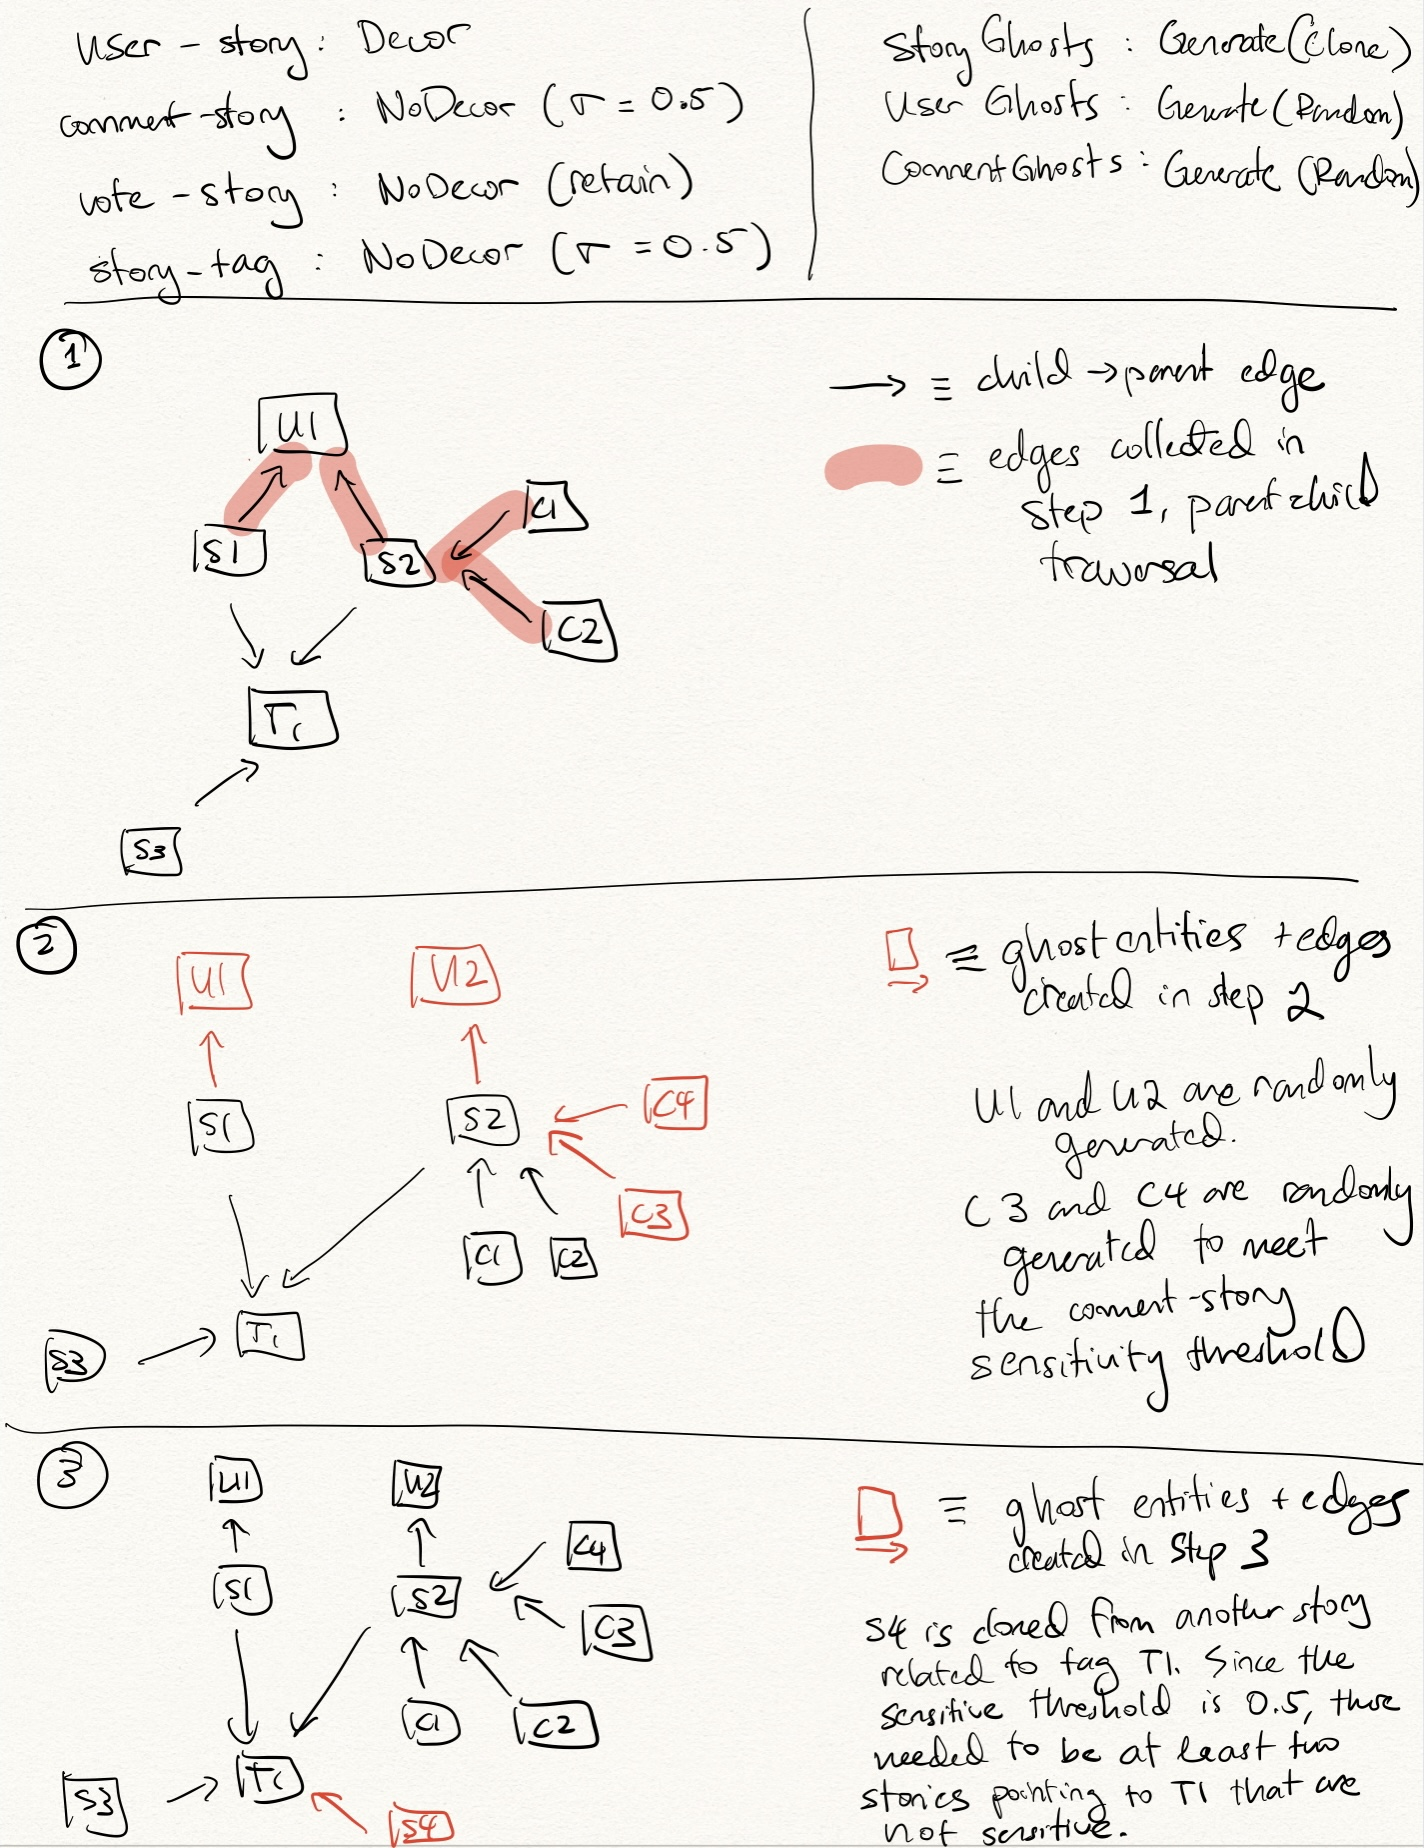
\includegraphics[width=.5\textwidth]{img/algo}
    \caption{Examples of \sys{}'s execution.}
    %different decorrelation policies. (a) full
    %decorrelation; (b) only direct user decorrelation; (c) decorrelation of stories clustered around tags with threshold 0.25}
\end{figure}

%\paragraph{Example policy.}
%We can imagine an application tin which only the sum of votes per story is ever queried by the application; clusters of
%votes around stories can therefore remain without leaking identifying information, and are thus
%assigned Policy 1, ``Do Not Decorrelate (Retain)''. 
%Decorrelation does propagate to the votes themselves, which are clustered by a \texttt{location} attribute; 
%this cluster by location can have a different decorrelation policy that generates ghost locations by
%randomizing the location, breaking up the cluster. 
%


\subsection{Maintaining aggregate accuracy.}
\sys{} optionally allows for entities to be decorrelated without affecting queries which
specifically return aggregation results.

Queries that specifically perform aggregations and return statistical measures (e.g.,
the count of number of users in the system, or the number of stories per user), can return
significantly different results. This affects the utility of the data for the application: for
example, if the application relies on the number of stories per tag to determine hot topics, these
would be heavily changed if ghost tags were created.  In addition, the adversary may learn which
entities are ghosts: for example, an abnormally low count of stories per tag might indicate to an
adversary that these tags are ghost tags.  \lyt{But perhaps it's ok if an adversary can tell what's
a ghost, as long as it can't tell which user each ghost is correlated with.}

\sys{} stores and separately updates answers to aggregation queries;
these answers are updated when queries update the data tables, and these queries do not read from
the application tables (which may contain ghost records).

An alternate solution might analyze the aggregations performed by application queries, and then
introduce ghosts that lead to the same (or close-enough) aggregation result. For example, if a tag
is split into ghost tags, one per story associated with the tag, but the application still would
like the count of stories for this tag to be high, one of the ghost tags can be populated with many
ghost stories to retain the count of stories per tag.  \sys{} would remove any ghost stories that
were created upon recorrelation. Note that this solution 1) requires that generating ghosts is
admissible, and 2) may be impossible for certain combinations of aggregations (e.g., queries that
return both the average stories per tag and also the total number of stories).

\lyt{I don't *think* differential privacy really should be applied here, because we'd also face the
issue of running out of privacy budget. Adding noise might ensure that the impact of any one
(real/ghost) user is very little, but it has its own noise/utility tradeoff. Furthermore, the amount
of noise necessary if many ghost users are created might be too large.}

\iffalse
\subsubsection{Modeling perfect decorrelation}
Application data is structured as tables, each representing a different \emph{data entity}, e.g.,\ a
story, user, or vote. Each entity type has a set of attributes, some of which are foreign keys to
other entities, and some of which are primitive column values.
Queries write, read from, and compute over entities.  All entities (e.g.,\
posts) that are correlated with the same attribute form a \emph{cluster}.
In database terms, entities in the same cluster belong to the same table, and the cluster is
identified by a shared foreign key or non-referencing column value.

Decorrelation of a user breaks any clusters identified by the user into singleton clusters, each
identified by a unique ghost user. In essence, the user is exploded into many ghost users, each
correlated with only one of the user's data entities and differing in its column
value attributes.

However, breaking up clusters around the user may not sufficiently decorrelate these entities from
the user. For example, stories belonging to the user may also cluster around a particular tag. Or
perhaps one of the user's stories is upvoted only by all of the users' friends (these upvotes
cluster around the story). These pieces of information allow an adversary to correlate a story back
to a single user, even when clusters around the user no longer exist.

The key observation here is that two types of clusters can still leak identifying information about
the user: (1) clusters identified by data entities owned by the users, and (2) clusters consisting
of the user's data entities, identified by other attributes (identity "proxies"). Decorrelation
recursively breaks up any such clusters into singletons by introducing ghost entities or attributes
(as was done with introducing ghost users), thus removing any identifying information leaked from
correlations between user's data entities and other entities in the application.

More generally, decorrelation continues to recursively break up any clusters that may recorrelate a
data entity back to the identifier of a broken-up cluster. Let $A$ be an attribute type (an entity
or a column value), and $B$ be an entity type. Let $a
\in A$ be the attribute being decorrelated. Given that $a$ identifies at least one cluster $B_a
\subseteq B$, decorrelation on $a$ does the following: 
\begin{enumerate} 
    \item \textbf{Break direct clusters and
            recurse.} $a$ splits into ghost entities $A_g \subseteq A$, one for each entity $b\in B_a$.
            Decorrelation then runs recursively on each cluster entity $b$.
            
            Furthermore, if the $A_g$ are in a cluster identified by some attribute $c$, $c$ is
            recursively decorrelated.
    \item \textbf{Break clusters around identity proxies and recurse.} If more than one of the
        $b \in B_a$ is also in a cluster that is identified by an attribute $c \in C$ (an identity
        ``proxy''), then we decorrelate $c$ from its data. 
        
\end{enumerate}
For example, each story (the $b$) posted by a user $a$ belongs in a cluster $B_a$ identified by $a$.
Decorrelation step (1) reassigns each story to a ghost user. Then each story is itself decorrelated.
If stories are decorrelated into a ghost story per vote, for example, then the votes would be
decorrelated. The ghost stories would cluster by the ghost user, so this ghost user would have to
further decorrelate.

Decorrelation step (2) may find that a particular tag $c$ identifies at least two of the users'
stories (these stories belong in a cluster $B_c$ identified by $c$). This tag is a column value
attribute, and not an entity specified by a foreign key. The tag is split into ghost tags, one per
user story, and because the tag itself has no attributes, decorrelation does not continue beyond the
tag.
\fi

